\chapter{Volumes with Integrals}
Suppose we wanted to know the volume of a theoretical irregular shape (we 
stipulate theoretical because, if you had this object and a large enough 
container, you could use displacement to determine the volume of the object). 

\section{Volume of a Sphere}
Below we will prove the volume of a sphere is given by $\frac{4}{3}\pi r^3$ 
using the integral method. Suppose we have a sphere of radius $r$ centered at 
the origin (see figure \ref{fig:sphere})

\begin{figure}[htbp]
\centering
    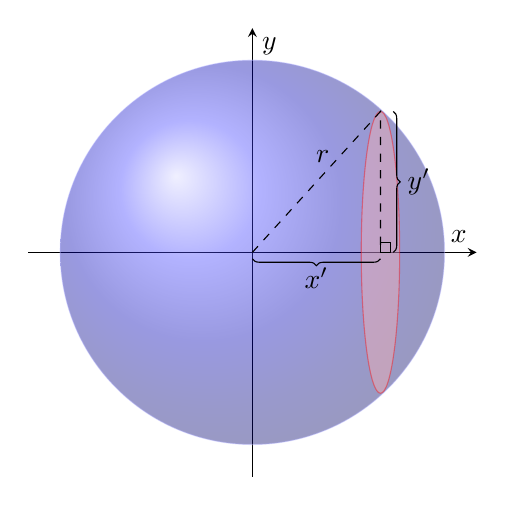
\begin{tikzpicture}
        \begin{axis}[xmin = -3.5, xmax = 3.5, ymin = -3.5, ymax = 3.5, axis lines = center, unit vector ratio=1 1 1, xtick = \empty, ytick = \empty, xlabel = $x$, ylabel = $y$]
            \draw[blue!30, shading = ball, ball color = blue, opacity= 0.4] (0,0) circle [radius = 3];
            \draw[red, fill = red!30, opacity = 0.4] (2, 0) ellipse [x radius = 0.3, y radius = 2.2];
            \draw[black, dashed] (0,0) -- (2, 2.2) -- (2, 0);
            \draw[black] (2, 0) rectangle (2.15, 0.15);
            \node[] at (1.1, 1.5) {$r$};
            \draw[decorate, decoration = {brace}] (2,-0.1) -- (0, -0.1); 
            \node[] at (1, -0.4) {$x'$};
            \draw[decorate, decoration = {brace}] (2.2, 2.2 ) -- (2.2, 0);
            \node[] at (2.6, 1.1) {$y'$};
        \end{axis}
    \end{tikzpicture}
    \caption{A vertical cross-section of a sphere}
    \label{fig:sphere}
\end{figure}

We begin by taking very thin vertical cross-sections. The radius of the 
cross-section is the height, $y$, of the sphere at the horizontal position, 
$x$. Since the edges of the cross-section lie on the sphere, we know the edge 
of the cross-section is distance $r$ from the origin. Applying the Pythagorean 
theorem, we see that $r^2 = x^2 + y^2$, which implies that $y = \sqrt{r^2 - x^2
}$. And then the area of the cross-section is given by $\pi y^2 = \pi (r^2 - x^
2)$. If we imagine each cross section as having a width, $dx$, and taking the 
sum of all the cross sections from $x = -r$ to $x = r$, we can write an 
integral equal to the volume of the sphere:
$$V_{sphere} = \int_{-r}^{r} \pi (r^2 - x^2)\,dx$$
And we can evaluate that integral:
$$V_{sphere} = \pi \int_{-r}^{r} r^2\,dx - \pi \int_{-r}^{r} x^2\,dx$$
$$V_{sphere} = \pi \left[ r^2 x \right] _{x = -r}^{x = r} - \frac{\pi}{3} \left[
x^3 \right] _{x = -r}^{x = r} $$
$$V_{sphere} = \pi \left[ r^3 - (-r^3) \right] - \frac{\pi}{3} \left[r^3 - (-r^
3) \right]$$
$$V_{sphere} = 2 \pi r^3 - \frac{2\pi}{3} r^3 = \frac{4}{3}\pi r^3$$

\section{Volumes of Solids of Revolution}
We can also find the volume of solids made by revolving a graph about the $x$ 
or $y$-axis. Suppose the graph $y = \sin{x}$ from $x = 0$ to $x = \frac{\pi}{2}$ were 
rotated vertically about the $x$-axis to form a solid. How could we find the 
volume of that solid? Well, we can imagine a rectangle of width $dx$ and 
height $y$ (see figure \ref{fig:sine_2d})

\begin{center}
\begin{figure}[htbp]
    \centering
    \begin{tikzpicture}
        \begin{axis}[axis lines = center, xmin = 0, xmax = 1.75, ymin = 0, 
        ymax = 1.05, clip = false]
          \addplot[name path = A, blue, thick, domain = 0:1.57, samples = 50]{sin(deg(x))}; 
          \addplot[name path = B, blue, thick] coordinates {(1.57, 0) (1.57, 1)};
          \addplot[blue!30, opacity = 0.4] fill between[ of = A and B];
          \filldraw[draw = red, fill = red!30, opacity = 0.4](1.1, 0) rectangle (1.13, 0.9); 
          \node[] at (1.115, -0.05) {$dx$};
          \draw[] (1.15, 0.01) -- (1.15, 0.89);
          \draw[] (1.14, 0.01) -- (1.16, 0.01);
          \draw[] (1.14, 0.89) -- (1.16, 0.89);
          \node[rotate = -90] at (1.21, 0.5) {height = $y = \sin{x}$};
        \end{axis}
    \end{tikzpicture}
    \caption{A cross section has width $dx$ and height $y = \sin{x}$}
    \label{fig:sine_2d}
\end{figure}
\end{center}

If we rotate the plot vertically about the $x$-axis, the rectangle becomes a 
cylinder with radius $y = \sin{x}$ and height $dx$ (see figure \ref{
fig:sine_3d}). And, therefore, the volume of each cylindrical slice is $V_{
slice} = \pi r^2 dx = \pi \cdot \sin^2{x} dx$. 

\begin{figure}[htbp]
\centering
    \begin{tikzpicture}
        \begin{axis}[axis lines = center, unit vector ratio=1 1 1, xtick = \empty, ytick = \empty, xlabel = $x$, ylabel = $y$]
        \addplot[name path = A, blue, thick, domain = 0:1.57, samples = 50]{sin(deg(x))}; 
        \addplot[name path = B, blue, thick, domain = 0:1.57, samples = 50]{-sin(deg(x))};
        \draw[blue, thick, fill = blue!30, opacity = 0.4] (1.57, 0) ellipse [x radius = 0.2, y radius = 1];
        \draw[red] (1, 0.841) arc [start angle = 90, end angle = 270, x radius = 0.1, y radius = 0.841];
        \draw[red, dashed] (1, -0.841) arc [start angle = -90, end angle = 90, x radius = 0.1, y radius = 0.841];
        \draw[red] (0.95, 0.841) arc [start angle = 90, end angle = 270, x radius = 0.1, y radius = 0.841];
        \draw[red] (0.95, 0.841) -- (1, 0.841);
        \draw[red] (0.95, -0.841) -- (1, -0.841);
        \node[] at (1, .9) {fixme shade graph};
        \end{axis}
    \end{tikzpicture}
    \caption{When rotated, the cross-section becomes a cylinder with radius $\sin{
	x}$ and width $dx$, which has a total volume of $\pi \sin^2{x} dx$}
    \label{fig:sine_3d}
\end{figure}

We can find the total volume by integrating from $0$ to $\pi$:
$$V = \int_0^{\pi/2} \pi \sin^2{x}\,dx$$
$$V = \pi \int_0^{\pi/2} \sin^2{x}\,dx$$

Recall the half angle formula, $\sin^2{x} = \frac{1}{2} \left( 1 - \cos{2x} 
\right)$. Substituting, we see that:
$$V = \frac{\pi}{2} \int_0^{\pi/2} \left( 1 - \cos{2x} \right)\,dx$$
$$V = \frac{\pi}{2} \left( x - \frac{1}{2}\sin{2x} \right)|_{x = 0}^{x = \pi/2}$$
$$V = \frac{\pi}{2} \left[ \left( \pi/2 - \frac{1}{2}\sin{\pi} \right) - \left(
0 - \frac{1}{2}\sin{0} \right) \right]$$
$$V = \frac{\pi}{2} \left[ \pi/2 - 0 - 0 + 0 \right] = \frac{\pi^2}{4}$$

\begin{Exercise}[label = volume1]
Find the volume of a solid created by rotating the region bounded by $x = 2
\sqrt{y}$, $x = 0$, and $y = 9$ about the $y$-axis. A graph is shown below.
 
\begin{tikzpicture}
	\begin{axis}[axis lines = center, ymin = -0.25, ymax = 9.25, xmin = -0.25, 
	xmax = 6, clip = false]
	    \addplot[name path = A, blue, thick, domain = 0:6]{(x/2)^2};
            \addplot[name path = B, blue, thick, domain = 0:6]{9};
            \addplot[blue!30, opacity = 0.4] fill between[
            of = A and B
            ];
            \draw[black] (0,5) ellipse (0.5cm and 0.2cm);
            \draw[-latex](-0.1, 4.67) -- (0.1, 4.67);
	\end{axis}
    \end{tikzpicture}  
\end{Exercise}

\begin{Answer}[ref = volume1]
If we are rotating about the $y$ axis, we should make our slices horizontal 
so their width is $dy$ (see graph below). Then the volume of each cylinder is 
given by $V = \pi r^2 dy$ and the total volume is given by:
$$V = \int_0^9 \pi \left[2 \sqrt{y} \right]^2\,dy$$
$$V = 4\pi \int_0^9 y\,dy = 2\pi y^2|_{y = 0}^{y = 9}$$
$$V = 2\pi \left(9 \right)^2 = 162\pi$$

\begin{tikzpicture}
	\begin{axis}[axis lines = center, ymin = -0.25, ymax = 9.25, xmin = -0.25, 
	xmax = 6, clip = false]
	    \addplot[name path = A, blue, thick, domain = 0:6]{(x/2)^2};
            \addplot[name path = B, blue, thick, domain = 0:6]{9};
            \addplot[blue!30, opacity = 0.4] fill between[
            of = A and B
            ];
            \draw[black] (0,5) ellipse (0.5cm and 0.2cm);
            \draw[-latex](-0.1, 4.67) -- (0.1, 4.67);
            \filldraw[draw = red, fill = red](0, 1.9) rectangle (2.828, 2);
            \draw[black](0.1, 2.2) -- (2.7, 2.2);
            \draw[black] (0.1, 2.1) -- (0.1, 2.3);
            \draw[black] (2.7, 2.1) -- (2.7, 2.3);
            \node[] at (1.5, 2.5) {radius = $2\sqrt{y}$};
            \draw[-latex] (4, 2.5) -- (2.9, 2);
            \node[] at (5, 2.7) {height = $dy$};
	\end{axis}
    \end{tikzpicture} 
\end{Answer}

\subsection{Using donuts for solids of revolution}
Sometimes there is space between the region we are rotating and the line we are
rotating it about. Consider the region bounded between $y = 2x$ and $y = x^2$  
(see figure \ref{fig:donut}):

\begin{center}
\begin{figure}[htbp]
    \centering
    \begin{tikzpicture}
        \begin{axis}[axis lines = center, xmin = 0, xmax = 2, ymin = 0, 
        ymax = 4, clip = false]
          \addplot[name path = A, blue, thick, domain = 0:2]{x^2};
          \addplot[name path = B, blue, thick, domain = 0:2]{2*x};
          \addplot[blue!30, opacity = 0.4] fill between [of = A and B];
          \draw[](1.2, 0) ellipse (0.2cm and 0.5cm);
          \draw[-latex](1.14, 0) -- (1.14, -0.1);
          \draw[draw = red, fill = red!30](1,1) rectangle (1.02, 2);
          \draw[red, dashed](1.01, 1) -- (1.01, 0);
        \end{axis}
    \end{tikzpicture}
    \caption{When rotated, the slices will become donuts with outer radius $2x$
    and inner radius $x^2$}
    \label{fig:donut}
\end{figure}
\end{center}

When rotated, the slices will take the form of donuts (or washers), the volume 
of which is $\pi \left( R^2 - r^2 \right) dx$, where $R$ is the outer radius 
and $r$ is the inner radius. Therefore, in this case, the total volume of the 
rotated region is given by:
$$V = \int_0^2 \pi \left[ \left( 2x \right)^2 - \left(x^2 \right)^2 \right]\,
dx$$
$$V = \pi \int_0^2 4x^2 - x^4\,dx = \pi \left[\frac{4}{3}x^3 - \frac{1}{5}x^5 
\right]_{x = 0}^{x = 2}$$
$$V = \pi \left[\frac{4}{3}2^3 - \frac{1}{5}2^5 \right] = \pi \left[ \frac{32}{
3} - \frac{32}{5} \right] $$
$$V = \frac{64 \pi}{15} $$

\begin{Exercise}[label = volume2]
What is the volume of the region bounded by $y = x^2$ and $y = 2\sqrt{x}$ when 
rotated about the $y$-axis? 
\end{Exercise}

\begin{Answer}[ref = volume 2]
First, since we are revolving around the $y$-axis, we know our slices will 
have width $dy$. We will re-write the functions as $x$ in terms of $y$:
$$x = \sqrt{y}$$
$$x = \frac{y^2}{4}$$
Setting them equal to each other to find the $y$-value at which they intercept:
$$\sqrt{y} = \frac{y^2}{4}$$
$$4 = \frac{y^2}{\sqrt{y}} = y^{3/2}$$
$$y = \sqrt[3]{4^2} = 2\sqrt[3]{2}$$
Examining a graph (shown below), we see that the outer radius is $x = \sqrt{y}$
and the inner radius is $x = \frac{y^2}{4}$. 

\begin{tikzpicture}
        \begin{axis}[axis lines = center, xmin = 0, xmax = 2, ymin = 0, 
        ymax = 3, clip = false]
          \addplot[name path = A, blue, thick, domain = 0:1.5874, samples = 50]
          {x^2}; 
          \addplot[name path = B, blue, thick, domain = 0:1.5874, samples = 100]
          {(2*sqrt(x)};
          \addplot[blue!30, opacity = 0.4] fill between[ of = A and B];
          \filldraw[draw = red, fill = red!30, opacity = 0.4](0.25, 1) rectangle 
          (1, 1.01); 
          \node[] at (1.115, 1.01) {$dy$};
          \draw[|-|] (0.03, 1.5) -- (0.53, 1.5);
          \draw[|-|] (0.585, 1.5) -- (1.2, 1.5);
          \node[] at (0.25, 1.7) {$r = \frac{y^2}{4}$};
          \node[] at (0.75, 2.5) {$R = \sqrt{y}$};
          \draw[-latex] (0.75, 2.4) -- (0.9, 1.55);
        \end{axis}
    \end{tikzpicture}

Then the total volume of the solid of revolution is given by:
$$V = \pi \int_0^{2\sqrt[3]{2}} \left(\sqrt{y} \right)^2 - \left( \frac{y^2}{4} 
\right)^2\,dy$$
$$V = \pi \int_0^{2\sqrt[3]{2}} \left[ y - \frac{y^4}{16} \right]\,dy$$
$$V = \pi \left[ \frac{1}{2}y^2 - \frac{1}{80}y^5 \right]_{y = 0}^{y = 
2\sqrt[3]{2}}$$
$$V = \pi \left[ \frac{6}{5} 2^{2/3} \right] \approx 5.9844$$
\end{Answer}

\section{Volumes of Other Solids}
You can also model a solid as a base defined by a function with cross-sections 
of specific shapes. Consider the function $y = x^2$ from $x = 0$ to $x = 2$ (
see figure \ref{fig:parab}). Suppose the area between the curve, the $y$-axis, 
and the line $y = 4$ defines a base and each vertical cross-section is a 
square. Then the width of the each cross section is $dx$, the length is $4 - 
x^2$, and (because they are squares) the height in the $z$-plane is also $4 - 
x^2$. Then the volume of each cross-section is $V_{slice} = \left(4 - x^2 
\right)^2 dx$ and the total volume of the solid is:
$$V = \int_0^2 \left(4 - x^2 \right) ^ 2\,dx$$
$$V = \int_0^2 \left( 16 - 8x^2 + x^4 \right)\,dx$$
$$V = \left[16x - \frac{8}{3}x^3 + \frac{1}{5}x^5 \right]_{x = 0}^{x = 2}$$
$$V = 16(2) - \frac{8}{3}(2)^3 + \frac{1}{5}(2)^5 = \frac{256}{15} 
\approx 17.067$$

\begin{figure}[htbp]
\centering
	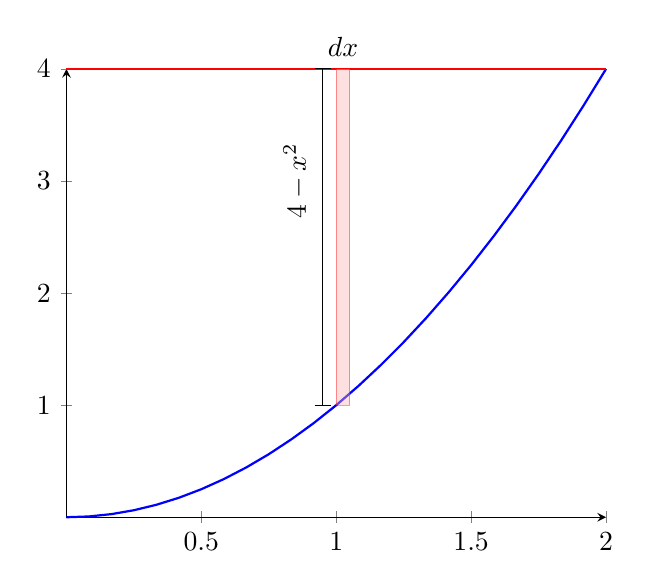
\begin{tikzpicture}
		\begin{axis}[axis lines = center, clip = false]
			\addplot[blue, thick, domain = 0:2]{x^2};
			\addplot[red, thick, domain = 0:2]{4};
			\filldraw[draw = red, fill = red!30, opacity = 0.4] (1, 1) rectangle (1.05, 4);
			\addplot[black] coordinates {(0.95, 4) (0.95, 1)};
			\addplot[black] coordinates {(0.92, 4) (0.98, 4)};
			\addplot[black] coordinates {(0.92, 1) (0.98, 1)};
			\node[rotate = 90] at (0.85, 3) {$4 - x^2$};
			\node[] at (1.025, 4.2) {$dx$};
		\end{axis}
	\end{tikzpicture}
	\caption{$y = x^2$ with a vertical cross-section}
	\label{fig:parab} 
\end{figure}

You can use a similar method for triangular, semi-circular, or any other shape 
cross-section. The trick is writing everything in terms of $x$ (when you cross 
sections are vertical and have width $dx$) or $y$ (when your cross section are 
horizontal and have length $dy$). 

\begin{Exercise}[label=AP_87]
[This question was originally presented as a multiple-choice, calculator-allowed 
question on the 2012 AP Calculus BC exam.] Let $R$ be the region in the first 
quadrant bounded above by the graph $y = \ln{(3 - x)}$, for $0 \leq x \leq 2$. 
$R$ is the base of a solid for which each cross section perpendicular to the 
$x$-axis is square. What is the volume of the solid? Give your answer to 3 
decimal places. 
\end{Exercise}

\begin{Answer}[ref=AP_87]
If each cross section is a square, then the volume of each cross section is 
given by $s^2 dx$, where $s$ is the side length of the square. Since the side 
length is equal to the distance between the graph of $y$ and the $x$-axis, we 
can see that $s = y = \ln{(3 - x)}$. And, therefore, the total volume of all 
the cross sections is given by $\int_0^2 \left[\ln{(3 - x)} \right]^2\,dx$. 
Using a calculator, this integral evaluates to $\approx 1.029$. 
\end{Answer}

